\subsection{Actual time spent working}

In a bureaucracy the actual time spent working is less than the number of hours you get paid for. Breaks during work, vacation from work, holidays, sick leave. 

% https://rescuetime.wpengine.com/work-life-balance-study-2019/

\begin{figure}
    \centering
    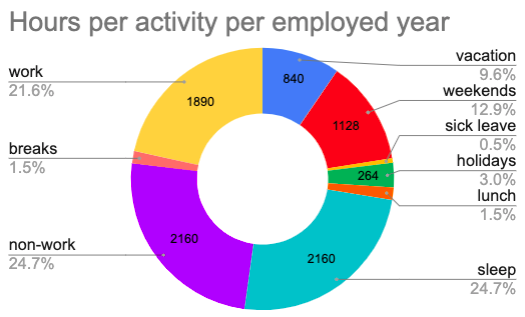
\includegraphics[width=0.8\textwidth]{images/hours_per_activity_per_employed_year}
    \caption{Hours of ``work'' per year when accounting for the rest of life. Assumes 5 weeks of vacation, 2 days of sick leave, and 11 holidays.}
    % footnotes in caption is not recommended; see https://texfaq.org/FAQ-ftncapt
    % however it can be done; see https://stackoverflow.com/questions/67621322/footnote-in-caption-of-figure-on-latex
    \label{fig:my_label}
\end{figure}

Fig~\ref{fig:my_label}
\footnote{\href{https://docs.google.com/spreadsheets/d/1ZaOZZXWkEzX4fFltUdlR4A6ENrAXnkzTW4YrjA4tDO8/edit?usp=sharing}{source for calculations}}